%!TEX program = xelatex
\documentclass[11pt,dvipsnames,table]{beamer}
\usepackage[no-math,cm-default]{fontspec}
\usepackage{amsmath}
\usepackage{amsthm}
\usepackage{amssymb}
\usepackage{CJK}
\usepackage{comment}
\usepackage{verbatim}
\usepackage{indentfirst}
\usepackage{syntonly}
\usepackage{fancyhdr}
\usepackage{xcolor}
\usepackage{graphicx}
%\usepackage{paralist}
\usepackage{beamerthemesplit}
\usepackage{euler}
\usepackage{ulem}
\usepackage{listings}
\usepackage{zhspacing}
\usepackage{booktabs}
\usepackage{multirow}
\usepackage{supertabular}
%\usepackage{mathptmx}

\usetheme{Berlin}
\usecolortheme{beaver}
\usefonttheme{professionalfonts}
%\setbeamerfont{section in toc}{size=\Large}
%\setbeamerfont{normal text}{size=9pt}
%\setbeamertemplate{headline}{}
%\setbeamertemplate{footline}{}

\defaultfontfeatures{Mapping=tex-text}
\zhspacing
%\setromanfont{Times New Roman}
\newfontfamily\zhfont[BoldFont=Adobe Heiti Std]{Adobe Song Std}
\setmonofont[Scale=1]{Courier New}
\XeTeXlinebreaklocale "zh"
\XeTeXlinebreakskip = 0pt plus 1pt

\lstset{language=C++,
	extendedchars=false,
	basicstyle=\ttfamily\tiny,
	keywordstyle=\color{blue},
	identifierstyle=\bfseries\color{blue!40!black}}

\setlength{\parindent}{2em}
\setlength{\baselineskip}{1.3\baselineskip}
%\linespread{1.3}

\setbeamercolor{math text}{fg=black}
\setbeamertemplate{qed symbol}{ $ \square $ }
\setbeamerfont{headline}{size=\fontsize{7.5pt}{\baselineskip}}
\setbeamerfont{footline}{size=\fontsize{7.5pt}{\baselineskip}}
\setbeamertemplate{theorems}[numbered]
\renewcommand{\thetheorem}{\arabic{subsubsection}.\arabic{theorem}}
\renewcommand{\thelemma}{\arabic{subsubsection}.\arabic{lemma}}
\newenvironment{qedframe}{%
	\begin{frame}[environment=qedqedframe]%
	}{%
	\qed
	\end{frame}%
}
\renewcommand{\appendixname}{结语}

\begin{document}

\title[趣题选讲]{\fontsize{20pt}{\baselineskip}趣题选讲}
\author[THU~CST~~胡泽聪]{THU~CST~~胡泽聪\\ Email:~huzecong@163.com}
\institute[THU~CST~~胡泽聪]{}
\date{}

\maketitle

{\fontsize{10pt}{\baselineskip}

\section{Intro}
\subsection{About me}
\begin{qedframe}
	\frametitle{关于我} \pause
	NOIp2011 二等奖 \pause
	\vskip 1em
	APIO2012 铜牌 \pause
	\vskip 1em
	WC2014 开幕式幸运奖
\end{qedframe}
\subsection{About this lesson}
\begin{qedframe}
	\frametitle{关于这次课程}
	题目来源:TC、CF、CC、ACM。
	\vskip 1em
	个人认为思路巧妙有趣的题。
	\vskip 1em
	分三个Part,难度递增(可能吧)。
\end{qedframe}

\section{Part I}
\subsection{2014 ACM/ICPC Asia Regional Xi'an Online - C}
	\begin{qedframe}
		\frametitle{Paint Pearls}
		给定一个长度为 $ n $ 的序列,每一位有一个目标颜色。初始时每一位都没有颜色。每次可以选择一个区间,将区间内的所有元素改为其\textbf{目标颜色}。设区间内不同颜色的数量为 $ x $ ,则操作的代价为 $ x^2 $ 。求最小代价。
		
		 $ n\leq 50000 $ 。
	\end{qedframe}
	\begin{qedframe}
		\frametitle{Paint Pearls - Solution}
		朴素的DP为:令 $ f[i] $ 表示前 $ i $ 个元素变为目标颜色的最小代价,方程为
		\[f[i]=\min\{f[j-1]+w(j,i)\}\]
		复杂度 $ O(n^2) $ 。
	\end{qedframe}
	\begin{qedframe}
		\frametitle{Paint Pearls - Solution}
		容易发现答案的上界为 $ n $ ---每次操作一个元素即可。 \pause
		
		基于上界又可以发现,如果一个区间内有超过 $ \sqrt{n} $ 种颜色,我们一定不会去操作它。 \pause
		
		换句话说,对于一个 $ f[i] $ ,只需要考虑 $ \sqrt{n} $ 个不同的 $ w(j,i) $ 的取值。 \pause
		
		而 $ f $ 显然单调不减,因此 $ w(j,i) $ 相同时选择最靠左的 $ f[j-1] $ 。 \pause
		
		我们只需知道这些 $ j $ 的值。
	\end{qedframe}
	\begin{qedframe}
		\frametitle{Paint Pearls - Solution}
		只要记录当前位置往左出现的前 $ \sqrt{n} $ 种颜色,及对应位置即可。
		
		移动到下一个数时,如果颜色出现在了前 $ \sqrt{n} $ 种之中,则暴力删除并移到最前面。
		
		总复杂度 $ O(n\sqrt{n}) $ 。 \pause
		\vskip 1em
		其实,数据中最优解选的每个区间都只有不超过5种颜色……
	\end{qedframe}
\subsection{2014 ACM/ICPC Asia Regional Beijing Online - E}
	\begin{qedframe}
		\frametitle{Explosion}
		 $ n $ 个房间,每个房间内可能有其他一些房门的钥匙。初始时所有房门都是锁上的。你决定随机炸门,问期望炸几次才能打开所有门。
		
		 $ n\leq 1000 $ 。
	\end{qedframe}
	\begin{qedframe}
		\frametitle{Explosion - Solution}
		形式化描述一下:
		
		 $ n $ 个点的有向图,每个点代表一个房间。如果 $ x $ 中有 $ y $ 的钥匙,那么 $ x $ 到 $ y $ 有一条有向边。炸开 $ x $ 则相当于删去 $ x $ 能到达的所有点。问期望删几次才能删掉整张图。
	\end{qedframe}
	\begin{qedframe}
		\frametitle{Explosion - Solution}
		考虑一个简单一些的问题:把有向图改成树(CF \#172 C)。 \pause
		\vskip 1em
		答案其实是
		\[\sum\frac{1}{depth_i}\]
		其中 $ depth_{root}=1 $ 。 \pause
		\vskip 1em
		由期望的线性性质,我们考虑每个点被删掉的概率。每个点只能被自己或自己的祖先删掉,其它点不会产生影响。那么点 $ i $ 被删一共 $ depth_i $ 种可能,其中只有一种可能是被自己删掉。而删掉的代价为 $ 1 $ ,因此总的期望就是上式。 \pause
		
		其实这并不是严谨的证明,但或许可以感受得到正确性吧= =
		
		严谨证明可以去看CF的题解。
	\end{qedframe}
	\begin{qedframe}
		\frametitle{Explosion - Solution}
		也就是说,我们只需知道每个点可以被多少点删掉,就能求出期望。。
		
		换言之,我们只要求出对于每个点,有多少个点可以到达它。
		
		对于树而言,这就是点的深度。对于一般的图呢? \pause
		\vskip 1em
		求出原图的强连通分量后,缩成一个DAG。
		
		之后用\texttt{bitset}等压位大法优化暴力。复杂度 $ O(n^3/32) $ 。似乎没有更好做法了。
	\end{qedframe}
\subsection{CodeForces Round \#221 (Div. 1) - C}
	\begin{frame}
		\frametitle{Circling Round Treasures}
		在一个 $ n\times m $ 的地图上,有一些障碍,还有 $ a $ 个宝箱和 $ b $ 个炸弹。你从 $ (sx,sy) $ 出发,走四连通的格子。你需要走一条闭合的路径,可以自交,且围出来的复杂多边形内不能包含任何炸弹。你围出来的复杂多边形中包含的宝箱的价值和就是你的收益。求最大收益。
		
		 $ n,m\leq 20 $ , $ a+b\leq 8 $ 。
		
		{\noindent
		\begin{figure}[h!]
			\centering
			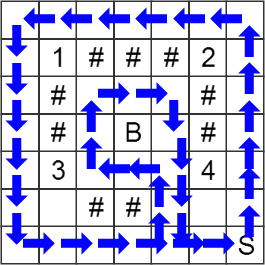
\includegraphics[width=3cm]{CF221.png}
		\end{figure}
		}
	\end{frame}
	\begin{qedframe}
		\frametitle{Circling Round Treasures - Solution}
		先考虑这个问题:如何判断一个点是否被复杂多边形所包含(不考虑在边上)? \pause
		\vskip 1em
		射线法。找一条由该点发出且不经过多边形上点的射线,然后看这条射线与多边形交了几次。如果交了奇数次,则在多边形内,否则在多边形外。 \pause
		\vskip 1em
		是否可以把这一方法用到这道题中?
	\end{qedframe}
	\begin{qedframe}
		\frametitle{Circling Round Treasures - Solution}
		其实是可以的。我们对于每个宝箱和炸弹维护一条射线,然后维护这些射线中哪些穿过了路径奇数次。 \pause
		
		令 $ f[x][y][k] $ 表示,当前在 $ (x,y) $ ,且集合 $ k $ 中的射线穿过了路径奇数次,这样的状态是否可行。
		
		转移时枚举下一步,然后看两步之间的线段穿过了哪些射线,并更新集合 $ k $ 。
		
		最后枚举所有集合 $ k $ ,要求炸弹的射线穿过路径偶数次,且 $ f[sx][sy][k]= $ \texttt{true}。用集合中宝箱的价值和更新答案。
		
		复杂度 $ O(nmk2^k) $ 。
	\end{qedframe}
\subsection{CodeForces Gym 100228 (ECNA2003) - I}
	\begin{qedframe}
		\frametitle{Graph of Inversions}
		对于长度为 $ n $ 的序列 $ a $ ,定义其逆序图 $ G $ 如下:无向图 $ G $ 有 $ n $ 个节点,编号为 $ 1\sim n $ ;对于任意的 $ 1\leq i<j\leq n $ ,如果有 $ a[i]>a[j] $ ,那么 $ G $ 中存在一条 $ i $ 和 $ j $ 之间的边。给定一个逆序图 $ G $ ,求 $ G $ 有多少个点集既是独立集又是覆盖集。
		
		 $ n\leq 1000 $ , $ 0\leq m\leq\frac{n(n-1)}{2} $ 。
	\end{qedframe}
	\begin{qedframe}
		\frametitle{Graph of Inversions - Solution}
		一般图的独立集问题是NP问题,因此逆序图肯定有良好的性质。 \pause
		
		不过逆序图也并非二分图,如序列 $ \{3,2,1\} $ 的逆序图就是一个奇环。所以把它当做图来做肯定是不靠谱的。我们不妨考虑逆序图对应的序列。
	\end{qedframe}
	\begin{qedframe}
		\frametitle{Graph of Inversions - Solution}
		可以发现,逆序图对应唯一的序列,两者之间存在一一对应关系。问题在于如何构造出这个序列。 \pause

		图中编号为 $ i $ 的节点即为序列中的第 $ i $ 个元素,一条边则代表一个逆序对。那么点 $ i $ 与所有编号大于 $ i $ 的点之间连的边数,就是序列中第 $ i $ 个数后面比 $ i $ 小的元素的个数。 \pause

		不难得出一个时间复杂度为 $ O(n^2) $ 的算法。
	\end{qedframe}
	\begin{qedframe}
		\frametitle{Graph of Inversions - Solution}
		独立集和覆盖集在原序列中对应什么? \pause
		
		独立集的点之间都不存在边,也就是说在序列中,选出来的子序列不构成逆序对。
		
		也就是说,选出来的应该是一个上升子序列。 \pause
		
		所有没有被选入覆盖集的点都与覆盖集中的至少一个点存在边相连。
		
		换句话说,对于序列中所有没有被选择的点,必须与至少一个被选择的点构成逆序对。
		
		也即,要么是选择了在它之前而且比它大的数,要么是选择了在它之后而且比它小的数。
	\end{qedframe}
	\begin{qedframe}
		\frametitle{Graph of Inversions - Solution}
		我们将两个条件结合起来考虑。 \pause
		
		我们将序列从被选择的点的位置切开,分成许多不同的段。假设某个段的左端点为 $ l $ ,右端点为 $ r $ , $ l $ 与 $ r $ 均为被选择的点。
		
		独立集要求选择一个上升子序列。那么覆盖集的条件等价于
		\[\forall i\in(l,r), a[i]<a[l]\textrm{或}a[i]>a[r]\]
	\end{qedframe}
	\begin{qedframe}
		\frametitle{Graph of Inversions - Solution}
		我们可以考虑这样的问题:假设目前被选择的子序列的结尾为点 $ i $ ,可以选择哪些点加入被选择的子序列?
		
		假设选择点 $ j $ ,那么应该满足:
		\[a[j]>a[i]\ \textrm{且}\ \min_{\substack{i<k<j\\a[k]>a[i]}}\{a[k]\}>a[j]\]
	\end{qedframe}
	\begin{qedframe}
		\frametitle{Graph of Inversions - Solution}
		基于上面的结论我们可以得到一个DP算法。令 $ f[i] $ 代表以第 $ i $ 位结尾的被选择子序列的方案数。
		
		为了处理方便,我们在序列的开头和结尾分别加上无穷小和无穷大,并强制选择这两个数。只要令 $ f[0]=1 $ 即可, $ f[n+1] $ 即为答案。转移方程则是
		\[f[j]=\sum_{\textrm{all valid }i}{f[i]}\]
		
		直接判断是否可行可以得到一个 $ O(n^3) $ 的算法。

		实际上没有必要直接判断。我们可以枚举 $ i $ ,然后向右枚举 $ j $ ,同时维护最小的满足条件的 $ k $ 。这样复杂度就成了 $ O(n^2) $ 。
	\end{qedframe}

\section{Part II}
\subsection{CodeChef January Challenge 2014 - FRBSUM}
	\begin{qedframe}
		\frametitle{ForbiddenSum} % 148
		定义一个多重集 $ S $ 的ForbiddenSum为,不能表示为 $ S $ 的某个子集中所有元素之和的最小元素。比如,多重集 $ \{1,1,3,7\} $ 的ForbiddenSum 为6。
		
		给定长度为 $ n $ 的序列 $ a $ ,有 $ m $ 次询问,每次给定 $ l_i $ 和 $ r_i $ ,询问多重集 $ S=\{a_l,a_{l+1},\ldots,a_r\} $ 的ForbiddenSum。
		
		 $ n,m\leq100000 $ , $ \sum{a_i}\leq10^9 $ 。
	\end{qedframe}
	\begin{qedframe}
		\frametitle{ForbiddenSum - Solution}
		有个问题和这个问题长得有点像: \pause
		
		\textbf{Subset Sum问题。}问是否存在给定集合的一个子集,使得子集中元素的和为给定的数。很遗憾这个问题是NP问题。因此二分答案判定什么的肯定是不行的。 \pause
		
		这个问题和Subset Sum问题的不同之处在于,这个问题只要求不能表示为Subset Sum的最小值。我们尝试从这个地方入手。
	\end{qedframe}
	\begin{qedframe}
		\frametitle{ForbiddenSum - Solution}
		对集合中的元素排序,记为 $ a_1,a_2,\ldots,a_n $ 。令 $ a_0=0 $ ,同时令 $ sum_i $ 为 $ a $ 的前缀和。
		
		再定义布尔值 $ f_i $ ,表示答案是否大于 $ sum_i $ 。 $ f_0 $ 显然为真。如何求出所有的 $ f_i $ ? \pause
		
		考虑从 $ f_{i-1} $ 推到 $ f_i $ 。如果 $ f_{i-1} $ 为假,显然 $ f_i $ 为假。否则,就意味着可以用 $ a_1,a_2,\ldots,a_{i-1} $ 凑出 $ 0\sim sum_{i-1} $ 的所有数。 \pause
		
		此时 $ f_i $ 为真就等价于,可以用 $ 0\sim sum_{i-1} $ 中的任意一个数以及 $ a_i $ 本身凑出 $ sum_{i-1}+1\sim sum_i $ 的所有数。这又等价于 $ a_i\leq sum_{i-1}+1 $ 。
		
		假设只有一次询问,我们可以对区间排序之后,在 $ O(n) $ 时间内求出所有 $ f_i $ 的值。记 $ p $ 为满足 $ f_p $ 为假的最小值,答案即为 $ sum_{p-1}+1 $ 。如果不存在这样的 $ p $ ,答案就是 $ sum_n+1 $ 。
	\end{qedframe}
	\begin{qedframe}
		\frametitle{ForbiddenSum - Solution}
		我们接着考虑怎么用数据结构优化这一过程。 \pause
		\vskip 1em
		套用区间无修改问题的万能做法---莫队算法。用平衡树维护当前区间中所有数的有序序列。对于每个节点,维护 $ v_i=a_i-sum_{i-1} $ ,以及子树中 $ v_i $ 的最大值 $ m_i $ 。我们要找的就是第一个 $ v_i>1 $ 的节点,这可以通过在平衡树中走一遍得出。 \pause
		
		这个算法的复杂度为 $ O(n\sqrt{n}\log n) $ ,而且常数较大,没有办法通过这道题。
	\end{qedframe}
	\begin{qedframe}
		\frametitle{ForbiddenSum - Solution}
		我们回到之前只有一次询问的暴力做法。我们能不能在这个算法上稍加优化? \pause
		\vskip 1em
		我们稍微改一下这个暴力做法。假设当前已知 $ f_i $ 为真,我们找到最大的满足 $ a_j\leq sum_i+1 $ 的 $ j $ ,显然有 $ f_j $ 为真。不断重复,直到能找到的最大的 $ j=i $ 。
		
		这个算法和之前的算法有什么区别? \pause
		\vskip 1em
		每次找最大的 $ j $ 可以用二分查找。而不难发现,每次 $ sum_j $ 至少会是 $ sum_i $ 的两倍,也即,最多查找 $ O(\log W) $ 次,其中 $ W $ 是权值。那么这个算法就是 $ O(\log n\log W) $ 的。
	\end{qedframe}
	\begin{qedframe}
		\frametitle{ForbiddenSum - Solution}
		我们再尝试用数据结构来优化这个新算法。 \pause
		\vskip 1em
		我们只需要查询,区间中权值在某个范围内的数之和。用可持久化线段树可以轻松做到单次查询 $ O(\log n) $ 。
		
		总复杂度 $ O(n\log n\log W) $ 。
	\end{qedframe}
\subsection{TopCoder SRM570 D1L3}
	\begin{frame}
		\frametitle{CurvyonRails}
		一块 $ n\times n $ 的地图,每个格子均为空地或者障碍。 
		
		现在要铺铁轨,每块空地都要被覆盖,每条路线必须闭合,且不能相交。
		
		有些空地上住着基佬,在这种空地上铺一块直的铁路需要花费1的代价。 
		
		给定地图,求是否能够铺铁轨,以及最小代价。
		
		{\noindent
		\begin{figure}[h!]
			\centering
			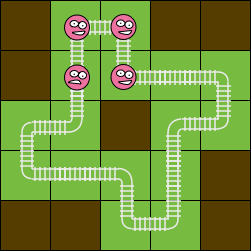
\includegraphics[width=2.5cm]{SRM570_1.png}
			\hskip 2em
			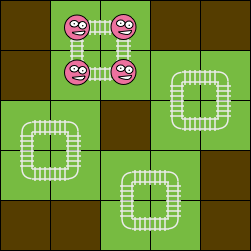
\includegraphics[width=2.5cm]{SRM570_2.png}
		\end{figure}
		}
	\end{frame}
	\begin{qedframe}
		\frametitle{CurvyonRails - Solution}
		第一眼看上去……插头DP? \pause
		\vskip 1em
		插头DP是会TLE的。
		
		这题和需要用插头DP的题有什么区别? \pause
		
		需要用插头DP的题对所求路径有特殊要求(比如为哈密尔顿回路),而且有些题需要求方案数。
		而此题只需覆盖每个格子,且所求为某个最小值。或许…… \pause
		\vskip 1em
		网络流?
	\end{qedframe}
	\begin{frame}
		\frametitle{CurvyonRails - Solution}
		先考虑判断是否有解。即,存在一些不相交不重复的回路可以覆盖所有空地且不覆盖任意障碍。 \pause
		
		也即,每个空地向相邻的空地连出恰好两条轨道。 \pause
		
		那么构建网络流模型。对地图(只考虑空地)黑白染色,从源向黑点、从白点向汇连容量为 $ 2 $ 的边。从黑点向相邻的白点连容量为1的边。满流即有解。
		
		{\noindent
		\begin{figure}[h!]
			\centering
			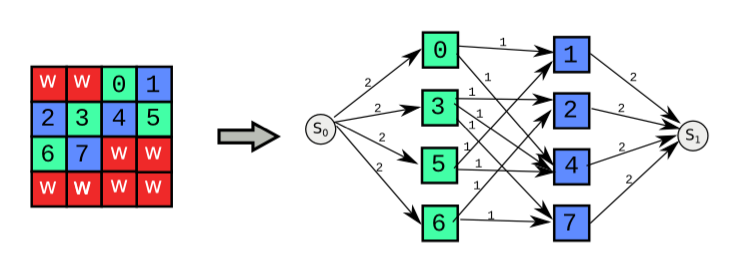
\includegraphics[width=7cm]{SRM570_3.png}
		\end{figure}
		}
	\end{frame}
	\begin{qedframe}
		\frametitle{CurvyonRails - Solution}
		那么弯的和直的铁轨怎么判断? \pause
		
		直的铁轨即,一块空地连出两条横向或纵向的轨道。
		
		弯的铁轨即,一块空地连出一条横向和一条纵向的轨道。 \pause
		
		先强制所有铁轨都是弯的,判断是否有解。
		
		在已有的网络流模型基础上改进。
		
		把每块空地拆成两个点,一个代表横向,一个代表纵向。
		
		横向点向横向相邻的空地的横向点连一条容量为 $ 1 $ 的边,纵向的类似。满流即有解。
	\end{qedframe}
	\begin{frame}
		\frametitle{CurvyonRails - Solution}
		{\noindent
		\begin{figure}[h!]
			\centering
			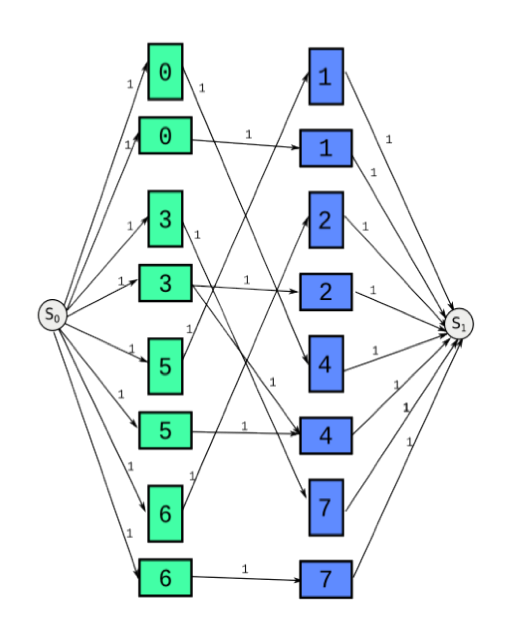
\includegraphics[width=5cm]{SRM570_4.png}
		\end{figure}
		}
	\end{frame}
	\begin{qedframe}
		\frametitle{CurvyonRails - Solution}
		如果要把一块铁轨改成直的呢? \pause
		
		如果是没人的空地,随便改;如果是有人的空地,收取费用。 \pause
		
		把网络流模型改成费用流模型,已有的边费用为 $ 0 $ 。
		
		在一块空地拆出的两个点之间连一条流量为1的双向边。
		
		如果空地有人,双向边的费用为 $ 1 $ ;否则为 $ 0 $ 。
		
		如果这类边有流量,就说明有一条轨道改变了方向。答案即为最小费用最大流。
	\end{qedframe}
	\begin{frame}
		\frametitle{CurvyonRails - Solution}
		{\noindent
		\begin{figure}[h!]
			\centering
			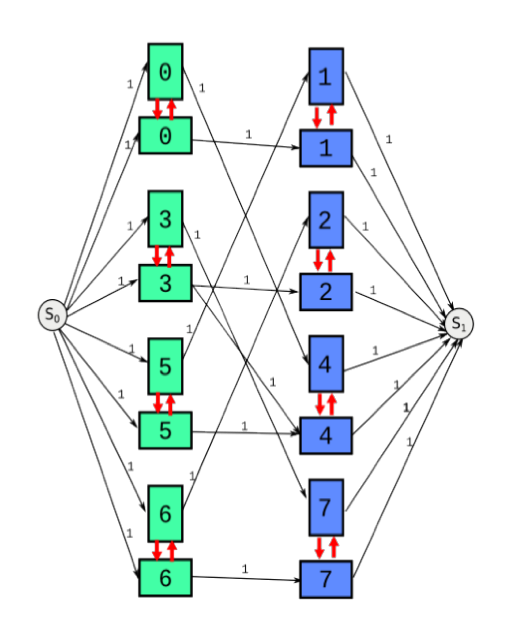
\includegraphics[width=5cm]{SRM570_5.png}
		\end{figure}
		}
	\end{frame}
\subsection{CodeChef March Challenge 2014 - GERALD07}
	\begin{qedframe}
		\frametitle{Chef and Graph Queries}
		给定一个 $ n $ 个点 $ m $ 条边的图,每条边编号为 $ 1\sim m $ 。有 $ q $ 次询问,每次给定 $ l $ 和 $ r $ ,询问当仅保留编号为 $ l\sim r $ 的边时,图中有多少个连通块。
		
		 $ n,m,q\leq 200000 $ 。可能有自环与重边。
	\end{qedframe}
	\begin{qedframe}
		\frametitle{Chef and Graph Queries - Solution}
		我们还是先看一个与之类似的问题:
		
		\textbf{AHOI2013~连通图}。与本题不同的是,每次询问只会删去最多 $ 4 $ 条边。而该题的做法是对询问分治。 \pause
		
		在本题中是行不通的,因为无法保证询问中删去的边(或保留的边)与询问数同阶。 \pause
		
		万能的莫队算法也难以实现,需要动态维护连通性。
	\end{qedframe}
	\begin{qedframe}
		\frametitle{Chef and Graph Queries - Solution}
		我们考虑按照 $ 1\sim m $ 的顺序依次向空图中加边。加入一条边时,只会有两种情况:
		\begin{enumerate}
			\item 合并了两个连通块;
			\item 形成了一个环。
		\end{enumerate} \pause
		
		先看第一种,只有合并两个连通块时才会产生贡献。我们要求的实际上就是一个区间中这类边有多少条。 \pause
		
		再看第二种,形成环则代表可以删去图中的一条边,并保持当前的连通性。
		
		不妨删去环上加入时间最早(即编号最小)的一条边。我们发现了什么?
	\end{qedframe}
	\begin{qedframe}
		\frametitle{Chef and Graph Queries - Solution}
		假设加入的边为 $ i $ ,删去的边为 $ a_i $ 。只有当 $ i $ 加入的时候才能``安全''删除 $ a_i $ ,否则会导致一个连通块分成两个。 \pause
		
		换句话说, $ i $ 会产生贡献 $ \iff $ 选择的区间中有 $ i $ 且没有 $ a_i $ 
	\end{qedframe}
	\begin{qedframe}
		\frametitle{Chef and Graph Queries - Solution}
		假设我们已求得 $ a $ 。当我们询问 $ [l,r] $ 时,我们实际上需要知道什么? \pause
		
		我们需要知道在 $ [l,r] $ 中有多少 $ a_i<l $ 。设其个数为 $ x $ ,连通块的个数就是 $ n-x $ 。 \pause
		
		用可持久化线段树可以轻松解决这一询问。
	\end{qedframe}
	\begin{qedframe}
		\frametitle{Chef and Graph Queries - Solution}
		至于求 $ a $ ,只需维护一棵LCT,按 $ 1\sim m $ 的顺序加边。
		
		加入一条边时,判断是否成环。如果构成了环,则找到环上编号最小的边的编号,即为 $ a_i $ 。
		
		如果没有成环,则记 $ a_i=0 $ 。注意当边为自环时, $ a_i=i $ 。
		
		总复杂度 $ O((n+m)\log n) $ 。
	\end{qedframe}

\section{Part III}
\subsection{CodeChef November Challenge 2013 - MONOPLOY}
	\begin{qedframe} % 21
		\frametitle{Gangsters of Treeland}
		给定一棵 $ n $ 个点的树, $ 1 $ 号节点为根。初始时每一个点都被染成了一种不同的颜色。如果一条边的两个端点颜色不同,则其费用为 $ 1 $ ,否则费用为 $ 0 $ 。
		
		有 $ q $ 次操作,操作有下面两种:
		\begin{itemize}
			\item 将从点 $ u $ 到根的路径上的所有点染成一种新的颜色。
			\item 询问点 $ u $ 子树中所有点走到根的费用的平均数。
		\end{itemize}
		
		 $ n,q\leq100000 $ 。
	\end{qedframe}
	\begin{qedframe}
		\frametitle{Gangsters of Treeland - Solution}
		直接维护每个点的颜色,查询时数链上有多少种不同的颜色? \pause
		
		带修改的树上第 $ k $ 大?或者是分块乱搞?无论哪个复杂度都太高。 \pause
		\vskip 1em
		为什么非得纠结颜色呢?可不可以利用``每次修改的颜色是一种新颜色''这样的性质?
	\end{qedframe}
	\begin{qedframe}
		\frametitle{Gangsters of Treeland - Solution}
		我们考虑直接维护边的费用。 \pause
		
		初始时所有边的费用均为 $ 1 $ ,修改一个点时,这个点到根的路径上的所有边的费用变为 $ 0 $ ,而其他和这条路径上的点相连的费用变为 $ 1 $ 。 \pause
		
		一次操作影响的边可能达到 $ O(n) $ ,直接操作是肯定不行的。一定还有别的性质。 \pause
		\vskip 1em
		每个点和儿子的连边中,至多一条费用为 $ 0 $ 。 \pause
		
		这似乎让人想起了什么……特别熟悉的东西…… \pause
		
		这不就是一棵Link-Cut Tree吗?
	\end{qedframe}
	\begin{qedframe}
		\frametitle{Gangsters of Treeland - Solution}
		费用为 $ 0 $ 的边就是LCT的实边,费用为 $ 1 $ 的边就是LCT的虚边。每次操作一个点就相当于expose(也称access)一个点。
		
		而一个点走到根的费用就是到根路径上的虚边条数。
		
		容易发现这个和原问题是等价的。 \pause
		\vskip 1em
		还记得LCT的复杂度吗?expose操作是均摊 $ O(\log n) $ 的。 \pause
		
		也就是说,expose时的``关键点'',即改变了实边的点,是均摊 $ O(\log n) $ 的。
		
		换言之,我们只有至多 $ O(n\log n) $ 次实质上的修改!
	\end{qedframe}
	\begin{qedframe}
		\frametitle{Gangsters of Treeland - Solution}
		我们实现一棵LCT,修改一个点时进行expose操作,每找到一个关键点就修改一次。
		
		而我们要维护的,就是每个点到根的虚边条数。 \pause
		
		这个就很简单了。求出DFS序之后建线段树,每次虚边和实边切换的时候就做一次段修改。查询则直接是段查询。
		
		总复杂度 $ O(n\log^2n) $ 。
	\end{qedframe}
	\begin{qedframe}
		\frametitle{Gangsters of Treeland - Extras}
		是不是觉得转化略神?
		
		实际上还可以更神。由于问题等价于LCT,我们可以增加其它LCT支持的操作,比如换根。 \pause
		
		回忆换根的实现:先把要提成根的点expose,再splay到根,之后再打翻转标记。那么我们可以给题目增加这么一个操作:换根,同时把新旧根之间的路径染成新的颜色。 \pause
		
		问题在于线段树那部分要怎么实现。我们需要支持子树查询、子树修改,以及换根。 \pause
		
		实际上也是可做的。这里就不说了,有兴趣的同学可以自己思考或者在课后与我交流。 \pause
		
		至于LCT的别的操作能不能支持呢?这个我没有细想,同样,有兴趣的同学可以自己思考这个问题。
	\end{qedframe}

\subsection{CodeChef June Challenge 2014 - SEAARC}
	\begin{qedframe}
		\frametitle{Sereja and Arcs}
		给定一个长度为 $ n $ 的序列 $ a $ ,对于任意的 $ x\neq y $ ,如果 $ a[x]=a[y] $ ,则在 $ x $ 和 $ y $ 之间画一条弧。称两条弧 $ x,y $ 和 $ l,r $ 相交当且仅当 $ x<l<y<r $ 或者 $ l<x<r<y $ 。求有多少条异色弧相交。
		
		 $ n\leq 100000 $ , $ a[i]\leq 100000 $ 。时限5s。
	\end{qedframe}
	\begin{qedframe}
		\frametitle{Sereja and Arcs - Solution}
		我们把圆弧视为线段,问题就是求有多少对有交且端点形如\texttt{1212}的异色线段。 \pause
		\vskip 1em
		将颜色按出现次数分类,次数大于 $ T $ 的为大块,其他的为小块。
		
		那么我们需要处理三种情况:
		\begin{enumerate}
			\item 大块之间的贡献;
			\item 小块与大块之间的贡献;
			\item 小块之间的贡献。
		\end{enumerate}
	\end{qedframe}
	\begin{qedframe}
		\frametitle{Sereja and Arcs - Solution}
		\textbf{大块之间的贡献} \pause

		我们枚举\texttt{1212}中的第二个\texttt{1},再枚举另外一种颜色。
		
		可以发现,答案为第二个\texttt{1}右边\texttt{2}的出现次数,乘上左边每个\texttt{2}的左侧的\texttt{1}的个数之和。 \pause
		
		由于大块个数不超过 $ O\left(\dfrac{n}{T}\right) $ ,我们可以预处理每个位置左侧每种颜色的出现次数。
		
		用这个就能维护,对于某种颜色 $ col $ ,和某个位置以左与这个位置颜色相同的所有位置,其左侧的 $ col $ 颜色的个数之和。
		
		计算时枚举一个位置和一种颜色。总复杂度 $ O\left(\dfrac{n^2}{T}\right) $ 。
	\end{qedframe}
	\begin{qedframe}
		\frametitle{Sereja and Arcs - Solution}
		\textbf{小块与大块之间的贡献} \pause

		枚举每个大块,再枚举每个小块。 \pause
		
		按照小块的每个元素把大块的元素划成若干区间,求出每个区间里的大块元素个数,记这个序列为 $ a $ 。
		
		假设我们枚举小块的左右端点,那么大块的两个元素的选择就是\texttt{(左边+右边)×中间}。
	\end{qedframe}
	\begin{qedframe}
		\frametitle{Sereja and Arcs - Solution}
		\textbf{小块与大块之间的贡献} \pause
		
		考虑当 $ a $ 的某一个元素成为``中间''部分时的贡献,我们需要求出这个元素为``中间''时可能的``左右''之和。
		
		这个元素左边第一块会被算一次,第二块被算两次,以此类推。整个这一部分还要再乘上右端点的可能的个数。
		
		右边也是类似的。这一部分是可以通过一些简单的预处理求出来的。
		
		那么复杂度也是 $ O\left(\dfrac{n^2}{T}\right) $ 。
	\end{qedframe}
	\begin{qedframe}
		\frametitle{Sereja and Arcs - Solution}
		\textbf{小块之间的贡献} \pause

		先考虑一个 $ O(n^3) $ 的算法,枚举\texttt{1212}中\texttt{2}的左右端点,再枚举另外一种颜色。
		
		此时相交的线段数就是该颜色在两个\texttt{2}之间的出现次数,乘上第一个\texttt{2}左边的出现次数。 \pause
		
		如果左端点从右往左扫,则可以在 $ O(1) $ 的时间内处理变化,并直接计算对答案的贡献的增量,从而优化到 $ O(n^2) $ 。 \pause
		
		令 $ f[i] $ 代表在当前右端点下,左端点为 $ i $ 时相交的线段数。不妨考虑,右端点右移时, $ f $ 会如何变化。
		
		如果我们能维护 $ f $ ,那么只需要枚举与右端点颜色相同的位置。
	\end{qedframe}
	\begin{qedframe}
		\frametitle{Sereja and Arcs - Solution}
		\textbf{小块之间的贡献} \pause
		
		我们考虑只枚举与右端点颜色相同的位置,此时对 $ f $ 的影响是按照这些位置分段的,每一段内的增量相同。
		
		也就是说,右端点右移会导致若干个段的修改,因此我们可以用树状数组维护答案。 \pause
		
		令 $ x_i $ 为颜色 $ i $ 的出现次数,复杂度应该是 $ O((\sum x^2_i)\log n) $ 。
		
		而 $ \max\left\{\sum x^2_i\right\} $ 其实是 $ O(nT) $ 级别的。
		
		考虑给某个 $ x_i $ 加 $ 1 $ 带来的增量 $ \Delta=2x_i+1 $ ,因此一定会选择最大的 $ x_i $ 去加1。
		
		换句话说,当有 $ \frac{n}{T} $ 个 $ x_i $ 为 $ T $ 时原式取到最大值。因此复杂度为 $ O(nT\log n) $ 。
	\end{qedframe}
	\begin{qedframe}
		\frametitle{Sereja and Arcs - Solution}
		综上,取
		\[T=\sqrt{\frac{n}{\log n}}\]
		可得最优复杂度 $ O(n\sqrt{n\log n}) $ 。时限有5s,毫无压力。 \pause
		
		但可以发现, $ O\left(\dfrac{n^2}{T}\right) $ 的有两个部分, $ O(nT\log n) $ 的只有一部分,因此应适当调大 $ T $ 。
		
		经过实测,取 $ T=\left\lfloor1.8\cdot\sqrt{\frac{n}{\log n}}\right\rfloor $ 时效果最好,只需要2.48s即可通过全部数据。
	\end{qedframe}

\appendix
\section{\appendixname}
\begin{frame}
	\frametitle{The End}
	\centering
	\LARGE
	谢谢大家!欢迎课后提问。
	\vskip 1em
	E-mail:~huzecong@163.com
\end{frame}
}

\end{document}
